\chapter{Неймовірне перетворення плати Arduino Uno у генератор імпульсів цікавої форми із частотою $\omega = 8 MHz$} 
\label{chap:second}

\section{Написання програми у середовищі Arduino IDE.}

Написання програми (рис. \ref{fig:code}) по суті зводиться до встановленя потрібних значень бітів регістрів, як описано у попередньому розділі. Тобто, встановлення СТС режиму шляхом присваювання біту WGM12 одиниці регістру TCCR1B, вибору режиму без дільника - присваювання одиниці біту CS10. Та подання на канал А (на arduino Uno вихід D9) високого рівня кожного разу, як встановлюється прапорець очистки регістру таймеру - біт COM1A0. Сама ж очистка відбувається як тільки значення регістру буде більшим за значення OCR1A. Тобто, таким чином можна отримати частоти вихідного сигналу 8, 8/2, 8/3 ... MHz. 
\begin{figure}[h]
\center{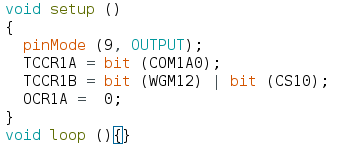
\includegraphics[width=0.6\linewidth]{code.png}}
\caption{Код програми.}
\label{fig:code}
\end{figure}

\section{Результати роботи}

\begin{figure}[h]
\center{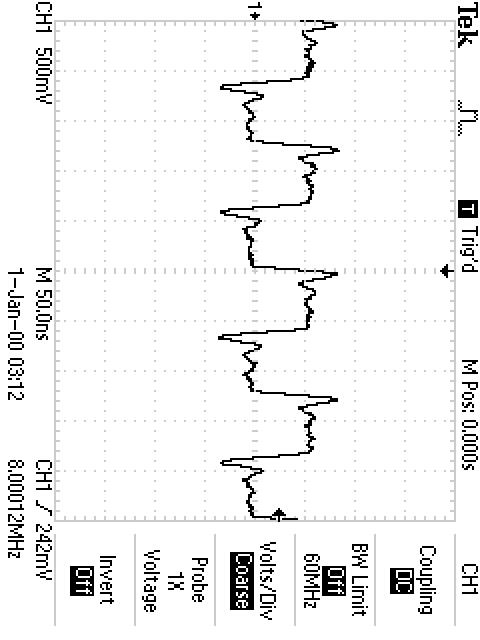
\includegraphics[angle=90,width=0.8\linewidth]{results.JPG}}
\caption{Покази осцилографа.}
\label{fig:results}
\end{figure}

Після прошивки плати arduino uno відповідним скетчем, та підключення осцилографа до відповідних ножок плати, було отримано картинку, зображену на рис. \ref{fig:results}. Дійсно було отримано сигнал, частота якого доходила до обіцяних $\omega=8 MHz = \omega_{gen}/2$, що є половиною від частоти вмонтованого у плату кварцового генератора. Звісно форма сигналу досить цікава, але її аналіз виходить за рамки цієї роботи. 

Також, потрібно звернути увагу на пусту функцію $loop()$ - можливість для використання такого генератора у будь-яких проектах

